\begin{frame}[label=caesar, fragile]{Wiederholung: Caesar \emoji{amphora}}
	\begin{minipage}[c]{.45\linewidth}
	    \begin{itemize}
	        \item Zwei Drehscheiben: Klartext aussen, Geheimtext innen
	        \item Schlüssel = Verschiebung der inneren Scheibe gegenüber A
	        \item Z.B.: HALLO = KDOOR
	        \item Extrem unsichere Verschlüsselung: Nur 25 mögliche Schlüssel
	        \item Einfacher als ausprobieren: Häufigkeitsanalyse
	    \end{itemize}
	    \end{minipage}
	    \begin{minipage}[c]{.45\linewidth}
	        \begin{figure}[H]
			     \centering
			     \resizebox{\linewidth}{!}{\Ceasar[10]}
			 \end{figure}
	    \end{minipage}
\end{frame}

\begin{frame}[label=caesarex, fragile]{Angriff auf Caesar}
	\centering
	Wie würden Sie folgenden Text knacken?\\[.5cm]
	    \defverbatim{\verbOne}{
\small\begin{verbatim}
Geheimtext: PKSGTJSAYYZKPUYKLQBKXRKASJKZNG...
\end{verbatim}
	        }
 \defverbatim{\verbTwo}{
	      \small\begin{verbatim}
  Klartext: JEMANDMUSSTEJOSEFKVERLEUMDETHA...
 Schlüssel: GGGGGGGGGGGGGGGGGGGGGGGGGGGGGG...
Geheimtext: PKSGTJSAYYZKPUYKLQBKXRKASJKZNG...
	      \end{verbatim}
	      }
	    \only<1-5>{\verbOne}
	    \only<2-4>{
	    Häufigster Buchstabe im obigen Geheimtext: \texttt{K}\\
	    Häufigster Buchstabe im deutschen Alphabet: \texttt{E}
	    }
	    
	 \only<3-5>{
	 \begin{itemize}
	   \item<3-5> \texttt{E} = Buchstabe 5
	   \item<4-5> \texttt{K} = Buchstabe 11
	   \item<5> Schlüssel = Verschiebung von 11-5 = 6 = Buchstabe \texttt{G}
	 \end{itemize}	 
	 }
	 \only<5-6>{
	 \centering\scalebox{.5}{\Ceasar[6]}
	 }
	 
	 \only<6>{\verbTwo}	
\end{frame}


\begin{frame}[label=vigenere, fragile]{Wiederholung letztes Mal: Vigenère \emoji{fleur-de-lis}}
\begin{verbatim}
  Klartext: JEM|AND|MUS|STE|JOS|EFK|VER|LE...
 Schlüssel: KEY|KEY|KEY|KEY|KEY|KEY|KEY|KE...
Geheimtext: TIK|KRB|WYQ|CXC|TSQ|OJI|FIP|VI...
\end{verbatim}
	
	\begin{itemize}
	    \item B=Verschiebung um 1 Position, C=Verschiebung um 2 Positionen, usw.
	    \item Allgemein: Verschiebung = $\text{Ord}(\square)$, wobei $\text{Ord}(A)=0$
	    \item 25 mögliche Schlüssel
	    \item Galt über 300 Jahre lang als sicher!
	\end{itemize}
	
	\begin{figure}[H]
      \centering
      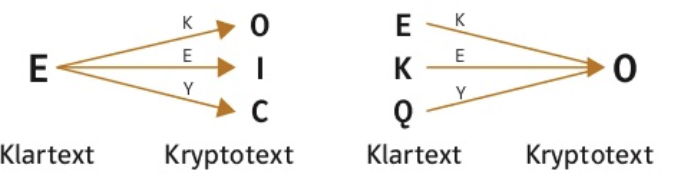
\includegraphics[width=.6\linewidth]{GrundlagenInfo/DataScience/03_Kryptologie/Figures/vigenere2.png}
	\end{figure}
\end{frame}



\begin{frame}[fragile]{Wiederholung letztes Mal: Angriff auf Vigenère}
	\texttt{MUZKJLQPAWJUMHYIILLCZAUPMRLZHLSVCMTZBCULGUPCIMPDQGTIP\\
		CQILVGYMGUBUJPNBMUZMNAPGYHNPKJLOTHBWSIVPWPKIHB}\\[.5cm]
	
	\begin{enumerate}
		\item<2-8> Schlüssellänge bestimmen $\rightarrow$ Friedmann'sche Charakteristik
		\begin{itemize}
			\scriptsize
			\item<2-8> 2 Gruppen: \texttt{\colorstring[ForestGreen,RoyalBlue]{MUZ KJL QPA WJU MHY IIL LCZ AUP MRL ZHL SVC 
							MTZ BCU LGU PCI MPD QGT IPC QIL VGY MGU BUJ 
							PNB MUZ MNA PGY HNP KJL OTH BWS IVP WPK IHB}}
			\item<3-8> 3 Gruppen: \texttt{\colorstring[ForestGreen,RoyalBlue,Crimson]{MUZ KJL QPA WJU MHY IIL LCZ AUP MRL ZHL SVC 
			MTZ BCU LGU PCI MPD QGT IPC QIL VGY MGU BUJ
			PNB MUZ MNA PGY HNP KJL OTH BWS IVP WPK IHB}}
			\item<4-8> 4 Gruppen: \texttt{\colorstring[ForestGreen,RoyalBlue,Crimson,LightSlateBlue]{MUZ KJL QPA WJU MHY IILLCZ AUP MRL ZHL SVC MTZ BCU LGU PCI MPD QGT IPC QIL VGY MGU BUJ PNB MUZ MNA PGY HNP KJL OTH BWS IVP WPK IHB}}
			\item<5-8> ...
		\end{itemize}
	\end{enumerate}
	
	\only<7>{
			$FC_T$ = Durchschnittliche Abweichung vom Mittelwert berechnen:
				\begin{figure}[H]
				        \centering
				        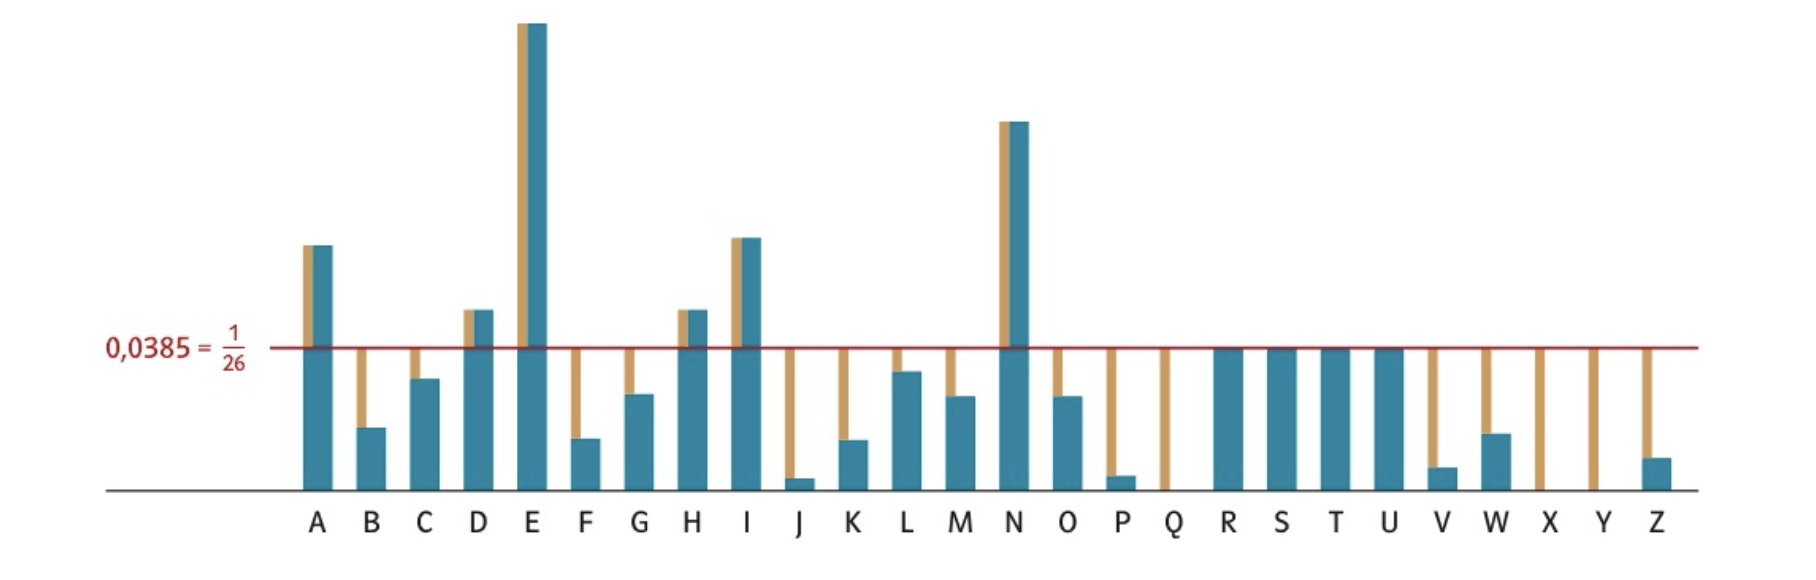
\includegraphics[width=.75\textwidth]{GrundlagenInfo/DataScience/03_Kryptologie/Figures/friedmann2.png}
				\end{figure}
				\scriptsize
				\begin{align*}
				    FC(T)&=\big(h_A(T)-\frac{1}{26}\big)^2+\big(h_B(T)-\frac{1}{26}\big)^2+\ldots+\big(h_Z(T)-\frac{1}{26}\big)^2
				\end{align*}
				\emoji{flag-germany} $FC(T)\sim 0.0388$ für deutsche Texte 
			}
		
	
	\only<8>{
		\begin{figure}[H]
			\centering
			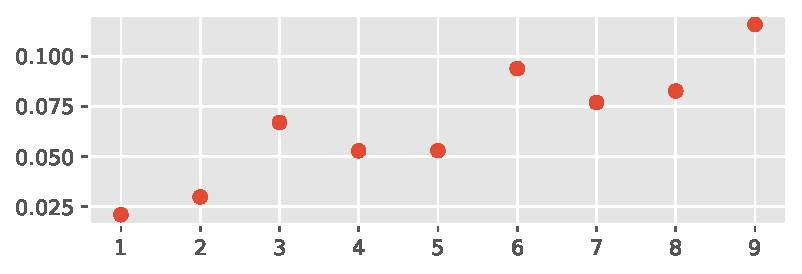
\includegraphics[width=.75\textwidth]{GrundlagenInfo/DataScience/03_Kryptologie/Figures/friedmann-ex3}
		\end{figure}
		$\rightarrow$ Zeigt, wie ungleich die Buchstaben verteilt sind, wenn wir sie in 1, 2, 3, 4... Gruppen aufteilen.
		}
\end{frame}

\begin{frame}{Wiederholung letztes Mal: Angriff auf Vigenère}
\texttt{\colorstring[ForestGreen,RoyalBlue,Crimson]{MUZ KJL QPA WJU MHY IIL LCZ AUP MRL ZHL SVC 
		MTZ BCU LGU PCI MPD QGT IPC QIL VGY MGU BUJ 
		PNB MUZ MNA PGY HNP KJL OTH BWS IVP WPK IHB}}
		
		$\rightarrow$ Häufigster Buchstaben pro Gruppe: \textcolor{ForestGreen}{M}, \textcolor{RoyalBlue}{G}, \textcolor{Crimson}{L}
		
		\begin{figure}[H]
			\centering
			\resizebox{.75\textwidth}{!}{\Ceasar[8] \Ceasar[2] \Ceasar[7]}
		\end{figure}
\end{frame}